\documentclass[14pt]{extbook}
\usepackage{multicol, enumerate, enumitem, hyperref, color, soul, setspace, parskip, fancyhdr} %General Packages
\usepackage{amssymb, amsthm, amsmath, latexsym, units, mathtools} %Math Packages
\everymath{\displaystyle} %All math in Display Style
% Packages with additional options
\usepackage[headsep=0.5cm,headheight=12pt, left=1 in,right= 1 in,top= 1 in,bottom= 1 in]{geometry}
\usepackage[usenames,dvipsnames]{xcolor}
\usepackage{dashrule}  % Package to use the command below to create lines between items
\newcommand{\litem}[1]{\item#1\hspace*{-1cm}\rule{\textwidth}{0.4pt}}
\pagestyle{fancy}
\lhead{Makeup Progress Quiz 3}
\chead{}
\rhead{Version C}
\lfoot{1648-1753}
\cfoot{}
\rfoot{Summer C 2021}
\begin{document}

\begin{enumerate}
\litem{
Which of the following functions \textit{could} be the graph below?
\begin{center}
    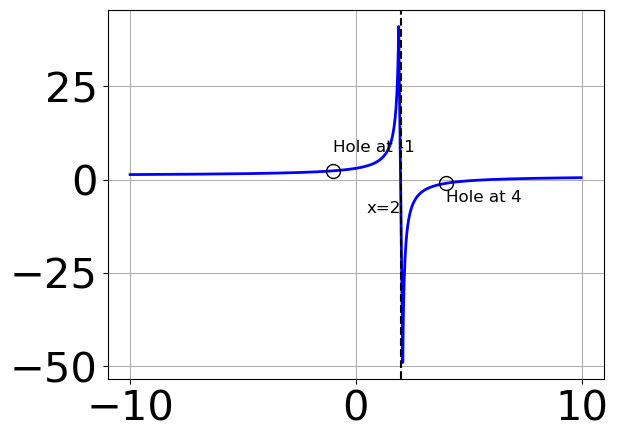
\includegraphics[width=0.5\textwidth]{../Figures/identifyGraphOfRationalFunctionC.png}
\end{center}
\begin{enumerate}[label=\Alph*.]
\item \( f(x)=\frac{x^{3} +7.0 x^{2} +14.0 x + 8.0}{x^{3} -12.0 x^{2} +41.0 x -30.0} \)
\item \( f(x)=\frac{x^{3} -9.0 x^{2} +20.0 x -12.0}{x^{3} +12.0 x^{2} +41.0 x + 30.0} \)
\item \( f(x)=\frac{x^{3} +5.0 x^{2} -8.0 x -12.0}{x^{3} +12.0 x^{2} +41.0 x + 30.0} \)
\item \( f(x)=\frac{x^{3} -5.0 x^{2} -8.0 x + 12.0}{x^{3} -12.0 x^{2} +41.0 x -30.0} \)
\item \( \text{None of the above are possible equations for the graph.} \)

\end{enumerate} }
\litem{
Determine the horizontal and/or oblique asymptotes in the rational function below.\[ f(x) = \frac{9x^{3} -39 x^{2} +52 x -20}{3x^{2} -14 x + 15} \]\begin{enumerate}[label=\Alph*.]
\item \( \text{Horizontal Asymptote of } y = 3.0 \text{ and Oblique Asymptote of } y = 3x + 1 \)
\item \( \text{Horizontal Asymptote of } y = 3.0  \)
\item \( \text{Horizontal Asymptote of } y = 3.0 \text{ and Oblique Asymptote of } y = 3x + 1 \)
\item \( \text{Horizontal Asymptote at } y = 3.0 \)
\item \( \text{Oblique Asymptote of } y = 3x + 1. \)

\end{enumerate} }
\litem{
Determine the vertical asymptotes and holes in the rational function below.\[ f(x) = \frac{12x^{3} -7 x^{2} -72 x -45}{6x^{2} -5 x -25} \]\begin{enumerate}[label=\Alph*.]
\item \( \text{Vertical Asymptotes of } x = 2.5 \text{ and } x = -0.75 \text{ with a hole at } x = -1.667 \)
\item \( \text{Vertical Asymptotes of } x = 2.5 \text{ and } x = -1.667 \text{ with no holes.} \)
\item \( \text{Vertical Asymptote of } x = 2.0 \text{ and hole at } x = -1.667 \)
\item \( \text{Holes at } x = 2.5 \text{ and } x = -1.667 \text{ with no vertical asymptotes.} \)
\item \( \text{Vertical Asymptote of } x = 2.5 \text{ and hole at } x = -1.667 \)

\end{enumerate} }
\litem{
Determine the horizontal and/or oblique asymptotes in the rational function below.\[ f(x) = \frac{3x^{2} +11 x -20}{9x^{3} -63 x^{2} +128 x -80} \]\begin{enumerate}[label=\Alph*.]
\item \( \text{Oblique Asymptote of } y = 3x -32. \)
\item \( \text{Horizontal Asymptote at } y = -5.000 \)
\item \( \text{Horizontal Asymptote of } y = 0.333  \)
\item \( \text{Horizontal Asymptote of } y = 0.333 \text{ and Oblique Asymptote of } y = 3x -32 \)
\item \( \text{Horizontal Asymptote of } y = 0 \)

\end{enumerate} }
\litem{
Which of the following functions \textit{could} be the graph below?
\begin{center}
    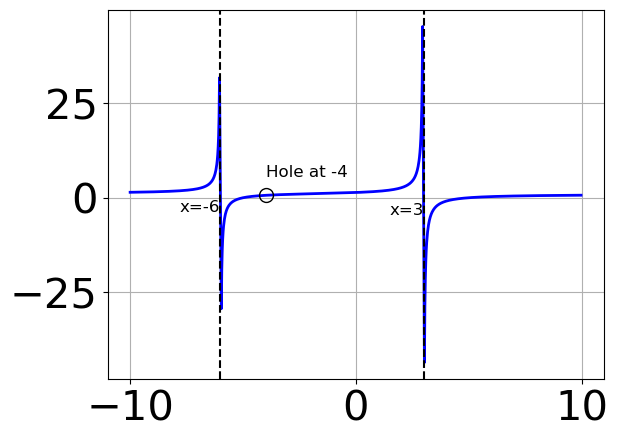
\includegraphics[width=0.5\textwidth]{../Figures/identifyGraphOfRationalFunctionCopyC.png}
\end{center}
\begin{enumerate}[label=\Alph*.]
\item \( f(x)=\frac{x^{3} +5.0 x^{2} -12.0 x -36.0}{x^{3} -2.0 x^{2} -33.0 x + 90.0} \)
\item \( f(x)=\frac{x^{3} -4.0 x^{2} -4.0 x + 16.0}{x^{3} +2.0 x^{2} -33.0 x -90.0} \)
\item \( f(x)=\frac{x^{3} +6.0 x^{2} +3.0 x -10.0}{x^{3} -2.0 x^{2} -33.0 x + 90.0} \)
\item \( f(x)=\frac{x^{3} -5.0 x^{2} -12.0 x + 36.0}{x^{3} +2.0 x^{2} -33.0 x -90.0} \)
\item \( \text{None of the above are possible equations for the graph.} \)

\end{enumerate} }
\litem{
Determine the horizontal and/or oblique asymptotes in the rational function below.\[ f(x) = \frac{4x^{2} +17 x -15}{20x^{3} +49 x^{2} -112 x + 48} \]\begin{enumerate}[label=\Alph*.]
\item \( \text{Horizontal Asymptote at } y = -5.000 \)
\item \( \text{Horizontal Asymptote of } y = 0 \)
\item \( \text{Oblique Asymptote of } y = 5x -9. \)
\item \( \text{Horizontal Asymptote of } y = 0.200 \text{ and Oblique Asymptote of } y = 5x -9 \)
\item \( \text{Horizontal Asymptote of } y = 0.200  \)

\end{enumerate} }
\litem{
Determine the vertical asymptotes and holes in the rational function below.\[ f(x) = \frac{12x^{3} -19 x^{2} -45 x -18}{12x^{2} +25 x + 12} \]\begin{enumerate}[label=\Alph*.]
\item \( \text{Vertical Asymptotes of } x = -1.333 \text{ and } x = -0.667 \text{ with a hole at } x = -0.75 \)
\item \( \text{Vertical Asymptotes of } x = -1.333 \text{ and } x = -0.75 \text{ with no holes.} \)
\item \( \text{Vertical Asymptote of } x = -1.333 \text{ and hole at } x = -0.75 \)
\item \( \text{Holes at } x = -1.333 \text{ and } x = -0.75 \text{ with no vertical asymptotes.} \)
\item \( \text{Vertical Asymptote of } x = 1.0 \text{ and hole at } x = -0.75 \)

\end{enumerate} }
\litem{
Determine the vertical asymptotes and holes in the rational function below.\[ f(x) = \frac{4x^{3} -12 x^{2} -7 x + 30}{6x^{2} -11 x -10} \]\begin{enumerate}[label=\Alph*.]
\item \( \text{Vertical Asymptotes of } x = -0.667 \text{ and } x = 2.5 \text{ with no holes.} \)
\item \( \text{Vertical Asymptotes of } x = -0.667 \text{ and } x = -1.5 \text{ with a hole at } x = 2.5 \)
\item \( \text{Vertical Asymptote of } x = -0.667 \text{ and hole at } x = 2.5 \)
\item \( \text{Vertical Asymptote of } x = 0.667 \text{ and hole at } x = 2.5 \)
\item \( \text{Holes at } x = -0.667 \text{ and } x = 2.5 \text{ with no vertical asymptotes.} \)

\end{enumerate} }
\litem{
Determine the vertical asymptotes and holes in the rational function below.\[ f(x) = \frac{6x^{3} +23 x^{2} -10 x -75}{4x^{2} +16 x + 15} \]\begin{enumerate}[label=\Alph*.]
\item \( \text{Vertical Asymptotes of } x = -1.5 \text{ and } x = -2.5 \text{ with no holes.} \)
\item \( \text{Holes at } x = -1.5 \text{ and } x = -2.5 \text{ with no vertical asymptotes.} \)
\item \( \text{Vertical Asymptotes of } x = -1.5 \text{ and } x = 1.667 \text{ with a hole at } x = -2.5 \)
\item \( \text{Vertical Asymptote of } x = 1.5 \text{ and hole at } x = -2.5 \)
\item \( \text{Vertical Asymptote of } x = -1.5 \text{ and hole at } x = -2.5 \)

\end{enumerate} }
\litem{
Determine the horizontal and/or oblique asymptotes in the rational function below.\[ f(x) = \frac{8x^{3} +26 x^{2} -5 x -50}{4x^{2} -25 x + 25} \]\begin{enumerate}[label=\Alph*.]
\item \( \text{Horizontal Asymptote at } y = 5.0 \)
\item \( \text{Horizontal Asymptote of } y = 2.0  \)
\item \( \text{Horizontal Asymptote of } y = 2.0 \text{ and Oblique Asymptote of } y = 2x + 19 \)
\item \( \text{Horizontal Asymptote of } y = 5.0 \text{ and Oblique Asymptote of } y = 2x + 19 \)
\item \( \text{Oblique Asymptote of } y = 2x + 19. \)

\end{enumerate} }
\end{enumerate}

\end{document}